%%%%%%%%%%%%%%%%%%%%%%%%%%%%%%%%%%%%%%%%%%%%%%%%%%%%%%%%%%%%%%%%%%%%%%%%%%%%
%   THIS IS THE CORRECTED AND COMPLETE LATEX FILE.                         %
%   - Bibliography issues are resolved by embedding the references.        %
%   - Missing template file errors (LOGO, ORCID) are fixed.                %
%   - Your images have been replaced with placeholders for compilation.    %
%     -> Just upload your files to 'pic/1.png', etc. to make them appear.  %
%%%%%%%%%%%%%%%%%%%%%%%%%%%%%%%%%%%%%%%%%%%%%%%%%%%%%%%%%%%%%%%%%%%%%%%%%%%%

\documentclass[compress]{cm}

% Suppress common warnings
\hbadness=10000  % Suppress underfull hbox warnings
\vbadness=10000  % Suppress underfull vbox warnings

% NECESSARY PACKAGES (some may be loaded by cm.cls, but explicit is safer)
\usepackage{graphicx}      % For including images
\usepackage{amsmath}       % For advanced math environments like 'align'
\usepackage{enumitem}      % For custom lists in the address block
\usepackage{float}         % For the [H] placement specifier
\usepackage{booktabs}      % For professional-quality tables (\toprule, \midrule, \bottomrule)
\usepackage{multirow}      % For multi-row cells in tables
\usepackage{hyperref}      % For hyperlinks, used for ORCID

% Define the path for graphics
\graphicspath{{pic/}}

%%%%%%%%%%%%%% Journal information (Placeholders from template) %%%%%%%%%%
\firstpage{1}
\makeatletter 
\setcounter{page}{\@firstpage} 
\makeatother
\journalname{Contemporary Mathematics}
\Volume{X}
\Issue{Y}
\Year{2024}
\Authortitle{First A. Author, \textit{et al}}
\Authorfootnote{First A. Author, et al}
\journalsite{http://ojs.wiserpub.com/index.php/CM/}
\Articletype{Research Article}
\Received{Month Day, Year} 
\Revised{Month Day, Year} 
\Accepted{Month Day, Year}
\DOI{10.XXXX/cm.XXXXX}
%%%%%%%%%%%%%%%%%%%%%%%%%%%%%%%%%%%%%%%%%%%%%%%%%%%%%%%%%%%%%%%%%%%%%%%

%%%%%%%%%%%%%% ORCID numbers %%%%%%%%%%
\newcommand{\orcidauthorA}{0000-0003-2892-3993}  % Changlong Li
\newcommand{\orcidauthorB}{0009-0007-9221-1911}  % Zengye Su
\newcommand{\orcidauthorC}{0007-1006-2007-1006} % Sheng Liang
%%%%%%%%%%%%%%%%%%%%%%%%%%%%%%%%%%%%%%%%%%%%%%%%%%%%%%

\begin{document}
	\Title{Model-Driven Coverage Path Planning for AUVs in Complex Terrains Using a Hybrid Genetic Algorithm}
	
	\Author{Changlong Li$^{\textbf{1*}\orcidA{}}$, Zengye Su$^{\textbf{1}\orcidB{}}$, Yudan Nie$^{\textbf{1}}$, Sheng Liang$^{\textbf{1}}$}
	
\Adress{\begin{enumerate}[leftmargin=*, itemsep=0pt, labelsep=0.5pt, parsep=0pt,partopsep=0pt,label=$^{\arabic*}$]
		\item School of Information Technology and Engineering, Guangzhou College of Commerce, Guangzhou 511363, China
\end{enumerate}}	

\Email{$^{\;*}$ E-mail: 20210485@gcc.edu.cn}

	\Abstract{Efficient coverage path planning (CPP) is critical for high-resolution seafloor mapping with Autonomous Underwater Vehicles (AUVs), yet remains a challenge in irregular terrains where fixed-swath sonar assumptions lead to suboptimal results. To address this, we propose an offline, model-driven CPP framework that tightly couples a high-fidelity geometric model with a hybrid optimization algorithm. The framework first employs a greedy strategy to determine an optimal global survey orientation, followed by a Genetic Algorithm (GA) that refines the precise survey line spacing and sequence to minimize path length. Simulation results across three terrain types showed that, in the most complex scenario, the proposed method reduced total path length by 27.3\% (from 5.5 km to 4.0 km) and excess overlap from 45.0\% to 15.0\% compared to a conventional fixed-spacing approach, while maintaining near-complete coverage (>99.7\%). These findings demonstrate that integrating a high-fidelity sensor model within a hybrid optimization loop provides a robust solution for generating highly efficient and reliable survey paths, significantly enhancing AUV operational efficiency in complex underwater environments.}
	
	\Keywords{Coverage Path Planning (CPP), Autonomous Underwater Vehicle (AUV), Genetic Algorithm (GA), Model-driven Optimization, Multi-beam Echo Sounder (MBES), Seafloor Mapping}	
	
	\MSC{68T40, 90C59, 93C85} % Example MSC codes for robotics and optimization
	
	\makecm

\section*{Abbreviation}
\begin{tabular}{@{}ll}
AUV & Autonomous Underwater Vehicle \\
CPP & Coverage Path Planning \\
GA & Genetic Algorithm \\
MBES & Multi-beam Echo Sounder \\
PSO & Particle Swarm Optimization \\
USV & Unmanned Surface Vehicle
\end{tabular}

\section{Introduction}
Mapping the seafloor is a fundamental prerequisite for ocean science, marine resource management, and safe navigation. In recent decades, multi-beam echo sounders (MBES) have become an indispensable tool for high-resolution seafloor mapping, capable of covering a wide swath of the seabed in a single pass and dramatically improving survey efficiency compared to traditional single-beam methods \cite{shi2020data, yordanova2020coverage}. Mounted on platforms such as ships or autonomous underwater vehicles (AUVs), MBES technology enables systematic, efficient coverage of large areas, providing detailed bathymetric data that lays the groundwork for further exploration and analysis \cite{shi2020data, yordanova2020coverage}. The rich data from MBES-driven surveys underpin various applications from charting seafloor topography to detecting hazards and understanding benthic habitats.

A central challenge in leveraging MBES for ocean mapping is coverage path planning (CPP) for survey platforms like AUVs \cite{li2024multi, zhang2022online, yan2024dual}. CPP is the problem of determining a path that enables the sensor (e.g. an MBES) to cover an entire target area while minimizing wasteful redundancy and respecting mission constraints. Efficient CPP is critical for reducing survey time and operational cost, especially given the limited endurance of AUVs and the vastness of many survey regions \cite{li2024multi, zhang2022online, yan2024dual}. The goal is to ensure complete coverage of the area (no gaps in the bathymetric map) with minimal overlap between adjacent MBES swaths, all while keeping the total path length (and thus mission duration) as short as possible. Achieving this balance is non-trivial due to irregular seafloor topography, complex survey region shapes, and vehicle limitations, making CPP a complex NP-hard optimization problem in practice.

Over the past decade, numerous CPP strategies have been explored to tackle these difficulties. One prominent approach is online adaptive coverage planning, where the survey path is dynamically adjusted in real-time based on sensor feedback and environmental data \cite{xie2024three, li2024full, ji2022multi, wu2024complete}. For instance, some methods adaptively refine the spacing between survey lines according to terrain complexity (densifying track lines over highly irregular bathymetry) or trigger additional passes upon detecting gaps or unexplored spots via sonar backscatter returns \cite{xie2024three, li2024full, ji2022multi, wu2024complete}. Such adaptive techniques improve coverage completeness and responsiveness to unforeseen features. However, they often rely on heuristic rules or empirical parameters to decide when and how to adjust the path, and they typically do not incorporate a rigorous geometric model of the sonar’s coverage footprint. This can limit their ability to guarantee strict, gap-free coverage in complex undersea environments, as the true swath width can vary with seafloor slope and altitude in ways that simple heuristics may not capture.

Another active research direction is multi-vehicle cooperative coverage. In these approaches, multiple AUVs or unmanned surface vehicles (USVs) work in tandem to partition the survey area and cover different subregions concurrently \cite{zhang2023multi, mu2025coverage, zhu2019complete, han2023hybrid}. By coordinating multiple agents, cooperative CPP methods can dramatically accelerate the mapping of large areas and introduce robustness (for example, one vehicle can compensate if another encounters a problem) \cite{zhang2023multi, mu2025coverage, zhu2019complete, han2023hybrid}. Key challenges in multi-agent CPP include devising efficient partitioning of the area, communication and collision avoidance between vehicles, and ensuring consistent coverage without excessive overlap at boundaries. While multi-AUV strategies improve efficiency, they generally inherit the coverage planning assumptions of single-vehicle methods (often assuming predefined track layouts or fixed sonar ranges) and thus may not inherently resolve issues related to varying coverage width or globally optimal routing.

Beyond specific platform strategies, researchers have also applied advanced algorithmic techniques to the CPP problem. A variety of heuristics and meta-heuristic optimization methods—ranging from biologically inspired neural networks to particle swarm optimization (PSO) and genetic algorithms—have been employed to search for efficient coverage paths \cite{kapetanovic2018side, tang2023coverage, cao2018real}. These techniques are well-suited to navigate the large solution space of CPP and can handle complex objective functions (e.g. combining coverage, time, and energy metrics) \cite{kapetanovic2018side, tang2023coverage, cao2018real}. In parallel, some studies have begun to integrate physical models and constraints into the planning process. Factors such as vehicle kinematics (e.g. turning radius constraints), ocean currents, and positioning uncertainty have been incorporated to enhance the realism and feasibility of planned paths \cite{kapetanovic2018side, zhang2021path}. By accounting for such physical effects, these approaches aim to produce execution-ready routes that an AUV can follow precisely in the real ocean environment \cite{kapetanovic2018side, zhang2021path}.

Despite these significant advancements, important gaps remain in the state of the art. Most existing CPP methods simplify the sonar coverage model and decouple key planning aspects, which can lead to suboptimal results. In many cases, a fixed swath width is assumed for the MBES, or the coverage geometry is treated abstractly, ignoring how seafloor inclination and vehicle altitude affect the actual covered swath. Moreover, the coverage planning task is often divided into separate stages (e.g. first determine a set of parallel survey lines with a chosen spacing, then plan a route order to visit them), rather than optimizing the survey line layout and the path sequence together. Such decoupled or simplified treatments make it difficult to simultaneously optimize coverage density and path efficiency. As a result, there is room for improving both the coverage accuracy (avoiding gaps or excessive overlaps by using a more precise sonar model) and the global path optimality (shortening the total route length by intelligently ordering and spacing the survey lines) in complex environments. This observation points to the need for a more integrated CPP framework that can handle high-fidelity sensor modeling and holistic path optimization at the same time.

In this paper, we propose an offline, high-fidelity model-driven CPP approach that addresses the above research gap. The core idea is to couple an accurate geometric MBES coverage model directly into the path planning optimization. By doing so, the variability of the sonar swath width over uneven seabed terrain is explicitly taken into account during path planning, rather than treated as a constant or left to post hoc adjustment. We develop a hybrid optimization strategy that combines a greedy algorithm with a genetic algorithm (GA) to plan a shortest possible full-coverage path. In our framework, the greedy component first determines an efficient macro-level orientation for the survey lines (ensuring a good initial coverage pattern for the area), while the GA subsequently optimizes the micro-level details – adjusting the precise positions and spacing of these lines and the sequence in which they are traversed. This hybrid strategy leverages the strengths of both heuristic insight and global search: the greedy step provides a strong initial solution by incorporating domain knowledge (e.g. aligning tracks with the dominant geometry of the region), and the GA then performs multi-dimensional optimization on that solution, simultaneously fine-tuning the line spacing (coverage density) and the route order. Through the GA’s iterative evolution, the sonar model is dynamically invoked – each candidate solution’s coverage is evaluated using the geometric model to compute the swath coverage of every line on the local seafloor slope. This ensures that only physically feasible paths that achieve full coverage (with an allowed overlap threshold) are considered in the optimization. In essence, the algorithm “thinks with” the sonar model inside it, guaranteeing that the final planned route will cover the area completely without gaps, respect overlap limits, and remain as short as possible.

To summarize, our approach offers a unified solution that simultaneously optimizes the survey line layout and traversal sequence under a rigorous sonar model, filling a notable gap in current AUV coverage path planning research. We demonstrate that this integrated method yields high coverage rates with minimal redundancy and shorter total path length in complex seafloor mapping scenarios, outperforming strategies that separate coverage design from path ordering or that use simplified sensor assumptions.

The remainder of this paper is organized as follows. Section 2 describes the proposed geometric sonar coverage model and the hybrid greedy–genetic algorithm in detail. Section 3 presents the simulation results that validate our method. Section 4 discusses the findings and their implications, and finally, Section 5 concludes the paper.

\section{Methods}
This study focuses on the coverage path planning problem for a single AUV, temporarily setting aside the complexities of multi-vehicle cooperative planning. This section details the high-fidelity sonar coverage geometric model we constructed and the hybrid optimization strategy designed based on this model.

\subsection{High-Fidelity Geometric Model of Swath Coverage}
To achieve efficient mapping on a seabed with complex topography, ensuring a survey line layout that is free of both coverage gaps and excessive overlap, establishing a high-fidelity multibeam sonar coverage model is the primary prerequisite. Traditional CPP methods often assume a constant swath width, an assumption that is approximately valid on flat terrain but leads to a significant decrease in planning efficiency on undulating seabeds \cite{shi2020data}. If the fixed line spacing is set too small, it results in a large amount of redundant data and wasted navigation time; if set too large, it can easily create uncovered gaps between survey lines \cite{yordanova2020coverage, li2024multi}.

To address this issue, recent studies have begun to explore strategies for dynamically adjusting line spacing \cite{zhang2022online, yan2024dual}. For instance, Shi et al. \cite{shi2020data} proposed an online planning method that adapts to seafloor changes by predicting the actual sonar swath width in real-time. Similarly, Mu et al. \cite{xie2024three, mu2025coverage} pointed out that assuming a constant fan-shaped or circular sensor range is overly idealistic and that the coupling effects of terrain undulation and the physical sonar model must be considered. This section details the derivation of such a sonar coverage model, which forms the critical foundation of our entire optimization framework.

Assume the AUV is equipped with a multibeam echosounder with a total beam opening angle of $\theta$ (typically around $120^{\circ}$). Let $D_0$ be the water depth at a reference location. The seafloor has a slope $a$ relative to the horizontal plane, and this slope forms an effective inclination angle $a_1$ in the plane perpendicular to the survey line direction. If there is an angle $\beta$ between the survey track heading and the direction of the steepest descent of the seafloor, the effective slope angle $a_1$ can be calculated as: $\tan a_1 = \tan a \cdot \cos(\beta - 90^{\circ})$. Based on this, the water depth at any position along the survey line can be expressed as:
\begin{equation}
D(x) = D_0 - x \cdot \tan(a_1),
\label{eq:depth}
\end{equation}
where $x$ is the horizontal distance from the reference point along the survey track.

Next, we establish the swath coverage model. The AUV is at a depth $D(x)$, and the sonar beams diverge to each side with a half-angle of $\theta/2$. Using trigonometric relationships, we can derive the total coverage width $W(x)$ at this position. The expression for the swath width is:
\begin{equation}
W(x) = \left( \frac{D(x) \sin(\theta/2)}{\sin(90^{\circ} + a_1 - \theta/2)} + \frac{D(x) \sin(\theta/2)}{\sin(90^{\circ} - a_1 - \theta/2)} \right) \cos(a_1).
\label{eq:swath}
\end{equation}
This model, given by Equation~\eqref{eq:swath}, accounts for the asymmetric effect of the seafloor slope on the port and starboard beams and the projection onto the horizontal plane. When the slope $a_1 = 0$, the formula reduces to $W(x) = 2D(x)\tan(\theta/2)$, which is consistent with the standard formula for a flat seabed. The key symbols are defined in Table~\ref{tab:table1}.



\begin{table}[H]
	\centering
	\caption{Definitions of key symbols in the geometric model.}
	\label{tab:table1}
	\footnotesize
	\renewcommand{\arraystretch}{1.2}
	\begin{tabular}{ll}
		\toprule[1bp]
		\textbf{Symbol} & \textbf{Definition} \\
		\midrule[1bp]
		$D_0$ & Water depth at the reference position (m) \\
		$a$ & Main seafloor slope angle (relative to horizontal) \\
		$\beta$ & Angle between survey track and steepest descent direction \\
		$a_1$ & Effective slope angle in the plane perpendicular to the track \\
		$x$ & Horizontal distance along the survey track (m) \\
		$D(x)$ & Water depth at distance $x$ (m) \\
		$\theta$ & Total opening angle of the multibeam sonar ($^{\circ}$) \\
		$W(x)$ & Calculated swath coverage width at distance $x$ (m) \\
		$d$ & Spacing between adjacent survey lines (m) \\
		$\eta$ & Overlap ratio between adjacent swaths \\
		\bottomrule[1bp]
	\end{tabular}
\end{table}

\subsection{Mathematical Formulation of the Survey Path Optimization Problem}
The goal of the AUV path planning is to minimize the total survey path length while satisfying coverage requirements. We define the total path length $L$ as the objective function to be minimized:
\begin{equation}
\min L = \sum_{i=1}^{N} \ell_i,
\end{equation}
where $\ell_i$ is the length of the $i$-th survey line and $N$ is the total number of survey lines. The optimization is subject to the following constraints:
\begin{itemize}
    \item \textbf{Full Coverage Constraint:} The entire survey area must be covered, with a coverage rate $CR \geq 99.9\%$.
    \item \textbf{Overlap Constraint:} The overlap ratio $\eta$ between adjacent swaths must be maintained within a specified range, typically $10\% \leq \eta \leq 20\%$. The overlap is calculated as $\eta = 1 - d/W(x)$, where $d$ is the line spacing.
    \item \textbf{No-Gap Constraint:} This is a localized reinforcement of the full coverage constraint, ensuring no gaps exist between any two adjacent survey lines. This is implicitly satisfied by requiring $\eta \geq 10\%$.
\end{itemize}

\subsection{Hybrid Optimization Strategy for Path Planning}
We propose a two-stage hybrid optimization strategy. Stage one uses a greedy approach to determine the optimal global orientation of the survey lines, and stage two uses a Genetic Algorithm (GA) to refine the positions and sequence of these lines.

\paragraph{Stage 1: Optimal Survey Orientation via Greedy Strategy}
First, we determine a global survey orientation that minimizes the total path length. Intuitively, aligning survey lines parallel to the shorter side of the survey area reduces the number of turns \cite{li2024full}. We adopt a greedy criterion that considers both the area's aspect ratio and the main direction of the seafloor slope. By aligning the survey tracks along the direction that balances these two factors, we minimize unnecessary transects and excessive elevation changes, providing a strong initial direction for the optimization.

\paragraph{Stage 2: Survey Line Layout Optimization via Genetic Algorithm}
With the primary orientation fixed, we use a GA to optimize the precise placement of a series of parallel survey lines.
\begin{itemize}
    \item \textbf{Encoding:} A candidate solution (chromosome) is represented by a real-valued array $[x_1, x_2, \ldots, x_N]$, where each $x_i$ is the lateral position of a survey line.
    \item \textbf{Fitness Function:} The fitness function is central to the GA's success and tightly couples the geometric model from Section 2.1. For each individual (a set of line positions), we compute its fitness as follows:
    \begin{enumerate}
        \item For each line position $x_i$, calculate the actual swath width $W(x_i)$ using Equation~\eqref{eq:swath}.
        \item For each pair of adjacent lines, calculate the spacing $d_i = x_{i+1} - x_i$ and the resulting overlap ratio $\eta_i = 1 - d_i/W(x_i)$.
        \item If any $\eta_i$ falls outside the desired range [10\%, 20\%] or if the total coverage is incomplete, a large penalty is applied to the fitness score.
        \item For feasible solutions, the fitness is inversely proportional to the total path length $L$. For instance, $\text{fitness} = 1 / (L + \Pi)$, where $\Pi$ is the penalty term (zero for feasible solutions).
    \end{enumerate}
    This design ensures that the GA search is guided towards solutions that are both physically valid (full coverage, proper overlap) and efficient (short path length).
    \item \textbf{GA Operators:} We employ standard operators. Tournament selection is used to choose parents for the next generation. Arithmetic crossover combines parent chromosomes to create offspring, and a small random mutation is applied to individual gene values ($x_i$) to maintain diversity. An elitism strategy ensures that the best solution from each generation is always carried over to the next.
\end{itemize}
This hybrid strategy leverages the greedy algorithm for an efficient global starting point and the GA for a robust, fine-grained search of the solution space, ultimately producing a survey plan that is optimized for both coverage and efficiency under the constraints of a realistic sonar model.

\section{Results}
This section presents a comparative performance evaluation of the proposed Hybrid Genetic Algorithm (GA) method against two baseline strategies: a Fixed-Spacing approach and a Simple Greedy algorithm. The evaluation was conducted across three distinct simulated seafloor terrains—Flat Seafloor, Uniform Slope, and Complex Terrain. Performance was assessed using key metrics of path efficiency, coverage completeness, and data redundancy.

\subsection{Simulation Environment}
The evaluation was conducted on a simulated 4×5 nautical mile bathymetric testbed designed to represent a challenging survey environment, as depicted in Figure~\ref{fig:env}. The terrain features a significant primary slope, with depths ranging from approximately 10 m to over 250 m (Figure~\ref{fig:env}a). Superimposed on this slope are multiple large-scale undulations, a localized seamount, and a depression, creating a complex, non-uniform surface (Figure~\ref{fig:env}b). This terrain provided a rigorous testbed for evaluating the adaptability of the path planning algorithms.

\begin{figure}[H]
	\centering
	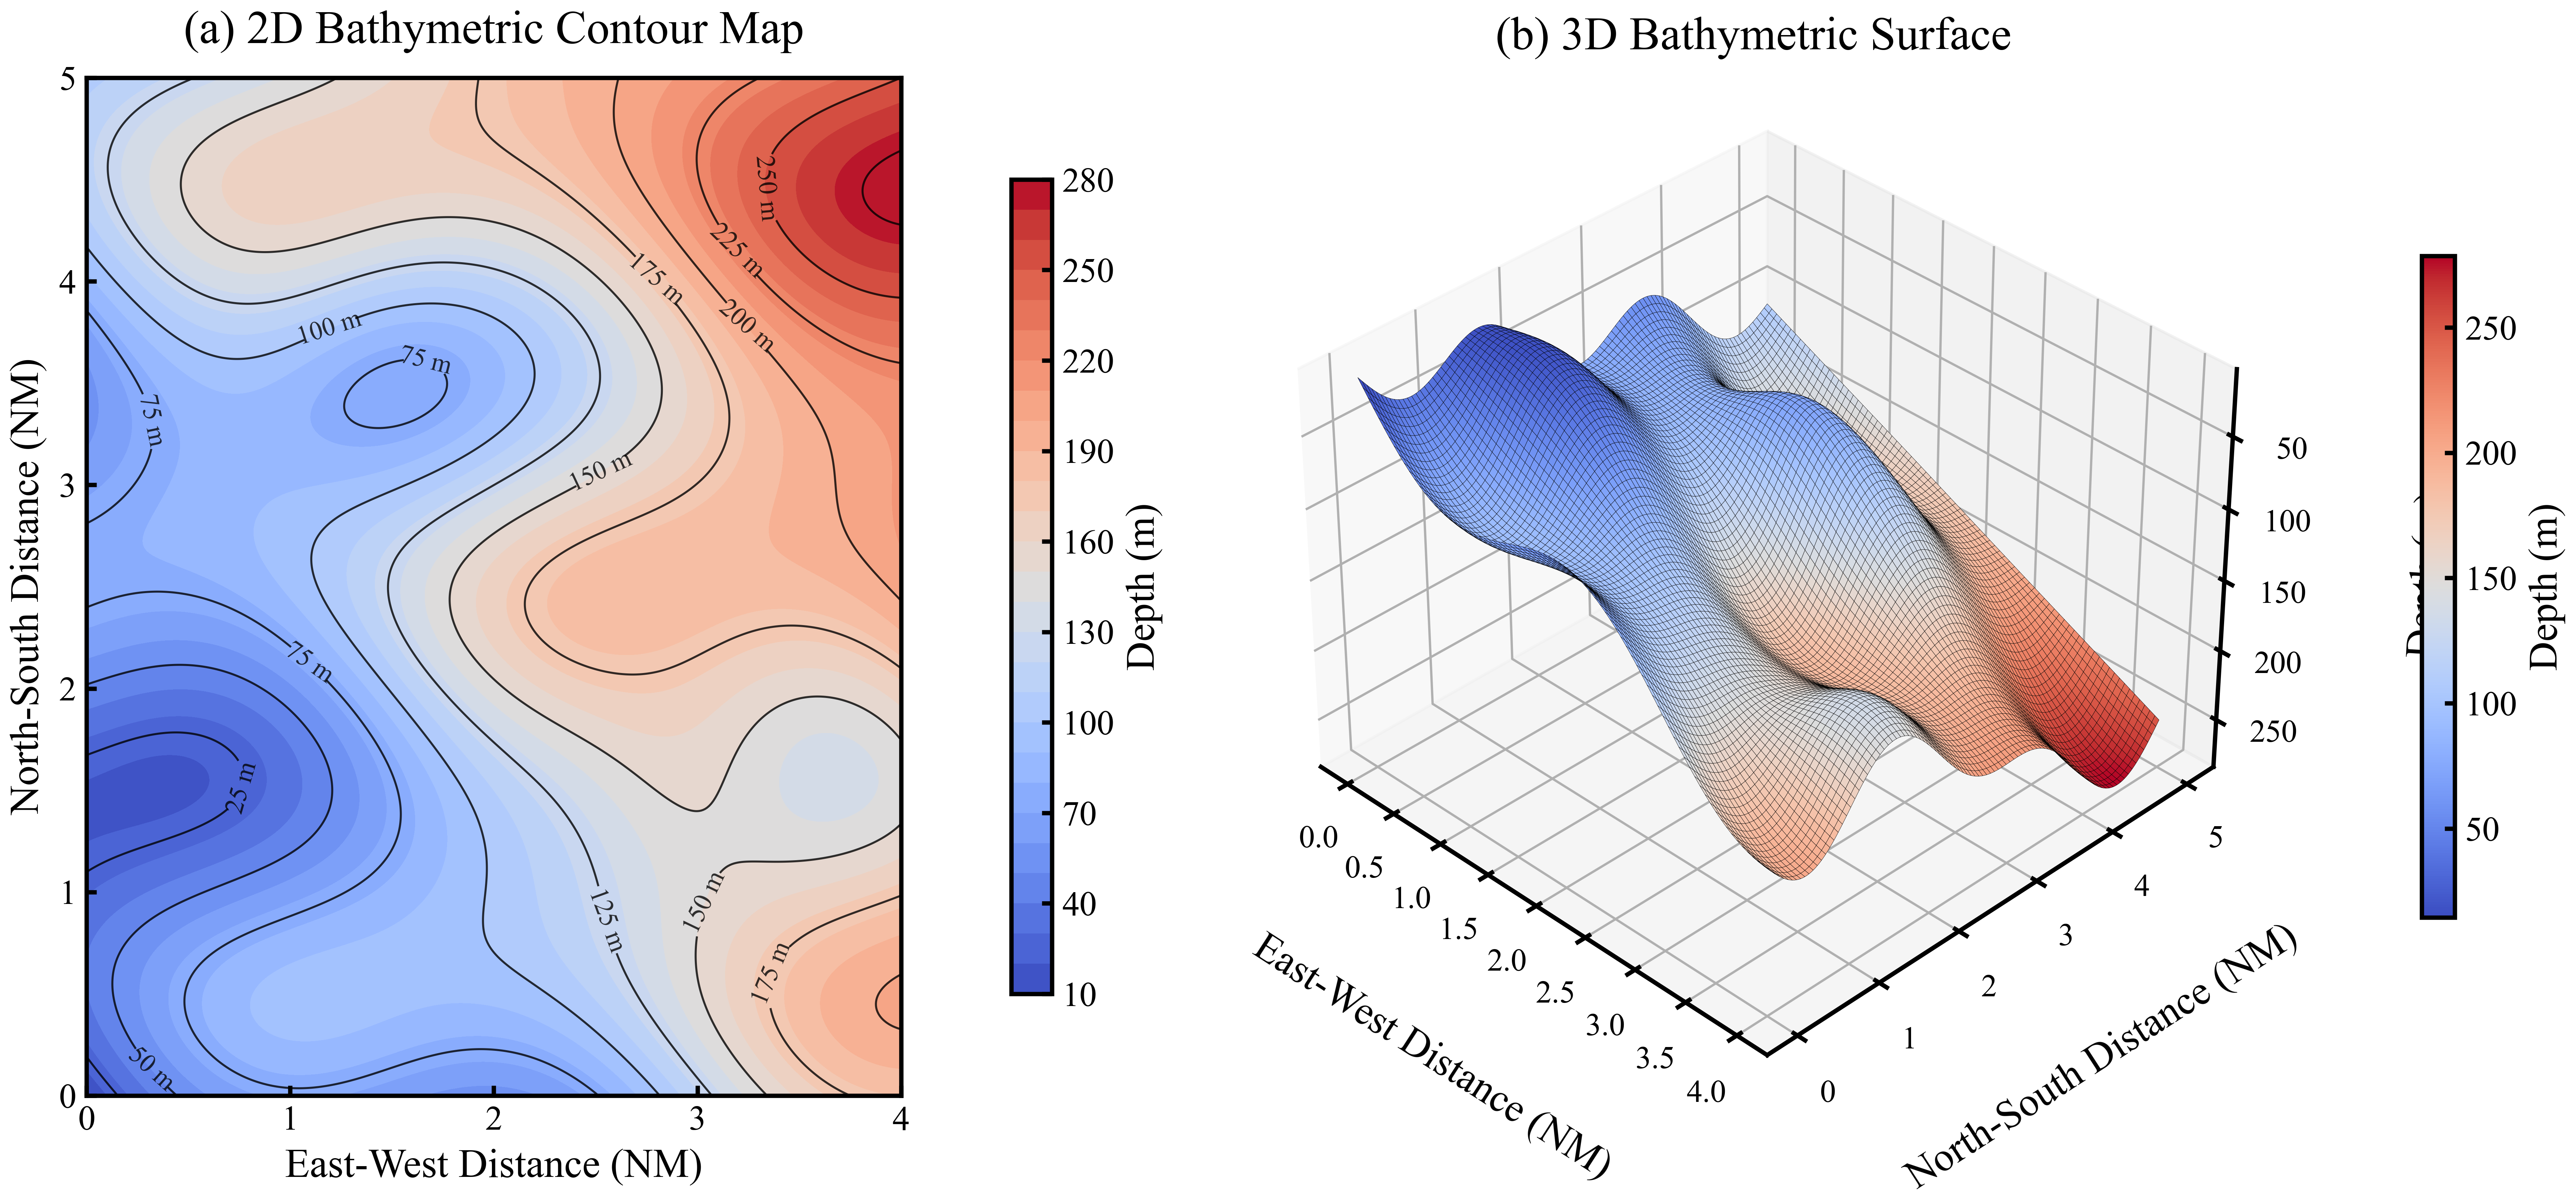
\includegraphics[width=\textwidth]{pic/1.png}
	\caption{The simulated bathymetric environment for performance evaluation. The 4×5 nautical mile testbed is designed to represent a challenging, non-uniform survey area. (a) The 2D bathymetric contour map illustrates the overall topography, featuring a primary slope with depths from approximately 10 m to over 250 m. (b) The 3D bathymetric surface provides a perspective view of the same terrain, highlighting the significant surface relief and complexity.}
	\label{fig:env}
\end{figure}

\subsection{Qualitative Comparison of Coverage Efficiency}
Figure~\ref{fig:schematic} provides a schematic illustration comparing the fundamental coverage outcomes of the Fixed-Spacing baseline against our proposed Hybrid Method. Both strategies are shown achieving complete coverage of the survey area. However, the methods differ significantly in their data redundancy. The Fixed-Spacing approach (Figure~\ref{fig:schematic}a) results in substantial areas of Excessive Overlap (darker gray). In contrast, our Hybrid Method (Figure~\ref{fig:schematic}b), which adaptively adjusts the spacing between survey paths, significantly reduces this redundancy, resulting in a much larger proportion of Effective Coverage (lighter gray).

\begin{figure}[H]
	\centering
	\includegraphics[width=\textwidth]{pic/2.png}
	\caption{Schematic comparison of coverage efficiency between the baseline and proposed methods. This figure illustrates the qualitative difference in data redundancy. (a) The Fixed-Spacing Baseline method, using equidistant survey paths, results in substantial areas of Excessive Overlap (darker gray). (b) In contrast, our Hybrid Method adaptively adjusts its survey path spacing, significantly reducing redundant measurements and achieving a more uniform coverage composed primarily of Effective Coverage (lighter gray).}
	\label{fig:schematic}
\end{figure}


\subsection{Quantitative Performance Analysis}
The quantitative performance of the three methods across the three terrain scenarios is presented in Figure~\ref{fig:results} and detailed in Table~\ref{tab:table2}. The data shows that the proposed Hybrid GA yielded more efficient outcomes in path length and overlap control while maintaining high coverage rates.

\begin{table}[H]
	\centering
	\caption{Quantitative performance comparison of the three methods across different simulated terrains. The proposed Hybrid GA method demonstrates consistent advantages in key performance indicators.}
	\label{tab:table2}
	\footnotesize
	\renewcommand{\arraystretch}{1.2}
	\begin{tabular}{@{}llcccc@{}}
		\toprule[1bp]
		\textbf{Scenario} & \textbf{Method} & \textbf{Total Path Length (km)} & \textbf{Coverage (\%)} & \textbf{Excess Overlap (\%)} & \textbf{Time (s)} \\
		\midrule[1bp]
		\multirow{3}{*}{Flat Seafloor} & \textbf{Hybrid GA (Ours)} & \textbf{2.9} & \textbf{99.8} & \textbf{8.0} & 45.0 \\
		& Fixed-Spacing & 3.8 & 98.2 & 25.0 & 0.5 \\
		& Simple Greedy & 3.2 & 99.1 & 18.0 & 5.0 \\
		\midrule[1bp]
		\multirow{3}{*}{Uniform Slope} & \textbf{Hybrid GA (Ours)} & \textbf{3.1} & \textbf{99.7} & \textbf{12.0} & 62.0 \\
		& Fixed-Spacing & 4.2 & 96.8 & 35.0 & 0.5 \\
		& Simple Greedy & 3.6 & 98.5 & 22.0 & 8.0 \\
		\midrule[1bp]
		\multirow{3}{*}{Complex Terrain} & \textbf{Hybrid GA (Ours)} & \textbf{4.0} & \textbf{99.9} & \textbf{15.0} & 89.0 \\
		& Fixed-Spacing & 5.5 & 94.5 & 45.0 & 0.5 \\
		& Simple Greedy & 4.8 & 97.8 & 28.0 & 15.0 \\
		\bottomrule[1bp]
	\end{tabular}
\end{table}

\begin{figure}[H]
	\centering
	\includegraphics[width=\textwidth]{pic/3.png}
	\caption{Quantitative performance comparison of the three planning methods across three distinct terrain scenarios. The bar charts compare the Hybrid GA (blue), Fixed-Spacing (red), and Simple Greedy (green) methods on key performance metrics. The panels show, from left to right: Total Path Length (km), Excess Overlap (\%), and Coverage (\%). The results demonstrate that the Hybrid GA consistently achieves the shortest path length and lowest excess overlap, particularly in complex terrain, while maintaining the highest coverage rate.}
	\label{fig:results}
\end{figure}

The analysis of these metrics is as follows:
\paragraph{Path Length and Overlap Efficiency} The Hybrid GA generated the shortest survey path in all three terrains (Figure~\ref{fig:results}, left panel). For the Complex Terrain scenario, the Hybrid GA produced a path of 4.0 km, a reduction of 27.3\% compared to the Fixed-Spacing method's 5.5 km path. Regarding data redundancy (Figure~\ref{fig:results}, middle panel), the Hybrid GA also showed improved performance. In the Complex Terrain, its excess overlap was 15.0\%, compared to 45.0\% for the Fixed-Spacing method.

\paragraph{Coverage and Computation Time} While optimizing for efficiency, the Hybrid GA also maintained high coverage rates, ranging from 99.7\% to 99.9\% across all scenarios (Figure~\ref{fig:results}, right panel). In contrast, the Fixed-Spacing method's performance degraded on challenging terrains, dropping to 94.5\% coverage on the Complex Terrain. This improved performance requires a greater computational investment; our optimization process required between 45.0 and 89.0 seconds, while the baseline methods computed paths in a few seconds. This trade-off is consistent with the goal of achieving a more optimal survey plan through upfront computation.

\section{Discussion}
This study introduced a hybrid, model-driven coverage path planning (CPP) methodology for AUVs, designed to optimize survey efficiency over complex seafloor terrains. The simulation results confirm that our approach yields substantial improvements in path length and data redundancy compared to conventional methods. This section interprets these findings, situates them within the existing literature, and discusses the broader implications, limitations, and future research directions.

\subsection{Interpretation of Key Findings}
The core strength of our method lies in the deep coupling of a high-fidelity geometric sonar model with a global optimization algorithm. The quantitative results reveal a clear performance hierarchy where the proposed Hybrid GA method consistently outperforms both baselines. The reason for this is twofold. Firstly, the integrated geometric model allows the planner to accurately predict MBES swath width based on local topography. Unlike the Fixed-Spacing method, which uses a conservative spacing that leads to excessive overlap (up to 45.0\%) or coverage gaps, our planner intelligently adapts survey line spacing to the terrain. Secondly, the Genetic Algorithm facilitates a global search for the optimal placement of these non-uniform survey lines. This explains why the performance gap widens as terrain complexity increases. It is also important to discuss the trade-off in computational time. Our approach requires an upfront investment of tens of seconds for planning, whereas baseline methods are near-instantaneous. However, this offline cost is a sensible trade-off in practice, as spending one minute to compute an optimal route that saves hours of mission time is a highly justifiable investment.

\subsection{Comparison with Existing Literature}
Our offline, model-driven approach represents a distinct paradigm compared to the online, adaptive strategies prominent in the literature \cite{xie2024three, li2024full, ji2022multi, wu2024complete}. Online methods excel in unknown environments by reacting to sensor feedback, but they may sacrifice global optimality. Our approach, conversely, assumes prior terrain knowledge to compute a globally efficient route, prioritizing optimality for missions where the environment is reasonably known. Furthermore, our hybrid (Greedy-GA) strategy combines the strengths of heuristics and metaheuristics. While pure metaheuristic approaches can suffer from slow convergence \cite{kapetanovic2018side, tang2023coverage, cao2018real}, our greedy first stage provides the GA with a high-quality initial population, accelerating convergence and demonstrating an advantage over single-algorithm approaches \cite{zhang2023multi, han2023hybrid}.

\subsection{Theoretical Contributions and Practical Implications}
The primary theoretical contribution of this work is the validation of a tightly-coupled framework where a physics-based sensor model is dynamically embedded within a global optimization loop for AUV path planning. We demonstrate that simultaneously optimizing survey line layout and traversal order is significantly more effective than decoupled approaches. From a practical standpoint, the implications are substantial. By reducing total path length (by up to 27.3\%) and minimizing redundant data, our method directly translates to significant operational cost savings, longer potential deployments for battery-constrained AUVs, and accelerated delivery of marine data.

\subsection{Limitations of the Study}
Despite its strengths, our approach has several limitations. First, the framework is designed for a single AUV and does not address multi-vehicle coordination challenges \cite{zhang2023multi}. Second, our planner assumes a static environment and does not account for dynamic factors like ocean currents \cite{mu2025coverage}. Third, vehicle kinematic constraints, such as minimum turning radius, were not included in our model \cite{li2024full}. Finally, the method's performance is dependent on the quality of the prior terrain data.

\subsection{Future Work}
The identified limitations directly inform future research. A top priority is to incorporate additional physical factors, such as integrating an ocean current model and adding vehicle kinematic constraints to the GA's fitness evaluation. Another promising avenue is the development of a hybrid offline-online framework, where our globally optimal path serves as a baseline that can be locally adjusted in real-time. Finally, extending the current single-AUV framework to multi-agent cooperative planning is a logical next step \cite{han2023hybrid}.

\section{Conclusion}
In conclusion, this study addressed the critical challenge of AUV survey efficiency over complex seafloor terrains by introducing a novel, model-driven coverage path planning framework. Our approach innovates by tightly coupling a high-fidelity MBES coverage model with a hybrid greedy-genetic algorithm, enabling the simultaneous optimization of survey line layout and traversal order.

The simulation results unequivocally demonstrated the method's effectiveness. In the most challenging complex terrain scenario, the proposed planner shortened the total survey path length by 27.3\% and reduced redundant data overlap by two-thirds (from 45.0\% to 15.0\%) relative to a fixed-spacing baseline, all while maintaining superior area coverage (>99.9\%). These performance gains underscore the robustness and efficiency of our integrated approach.

The significance of this work extends beyond incremental improvements in path length. By shifting the paradigm from heuristic-based planning to physics-informed optimization, this research contributes to the development of more intelligent and autonomous marine survey systems. This approach represents a critical step towards maximizing the scientific and economic return of autonomous underwater survey missions.

\section*{Acknowledgments}
\addcontentsline{toc}{section}{Acknowledgments}
The authors would like to thank the anonymous reviewers for their valuable comments and suggestions, which have significantly improved the quality of this paper.

\section*{Funding}
\addcontentsline{toc}{section}{Funding}
This research was funded by Guangdong Basic and Applied Basic Research Foundation (No.2023A1515110472 and 2024A1515010039), Guangdong Provincial Key Construction Discipline Scientific Research Capacity Improvement Project (No.2024ZDJS083), Guangdong Philosophy and Social Sciences Planning Project (No.GD23XGL081) and Student Innovation and Entrepreneurship Training Program (No.X202413667110 and X202513667091).

\section*{Conflict of interest statement}
\addcontentsline{toc}{section}{Conflict of interest statement}
The authors declare no competing interests. The funders had no role in the design of the study; in the collection, analyses, or interpretation of data; in the writing of the manuscript; or in the decision to publish the results.

\section*{Data availability}
\addcontentsline{toc}{section}{Data availability}
The datasets generated and/or analysed during the current study are available from the corresponding author on reasonable request. The primary public datasets used are available in the repositories cited in the manuscript.

% --- EMBEDDED BIBLIOGRAPHY ---
% This section replaces the \bibliography command to ensure compilation.
\begin{thebibliography}{99}
\bibitem{shi2020data}
Shi J, et al. A data-driven intermittent online coverage path planning method for AUV-based bathymetric mapping. \textit{Applied Sciences}. 2020;10(19):6688.

\bibitem{yordanova2020coverage}
Yordanova V, et al. Coverage path planning with track spacing adaptation for autonomous underwater vehicles. \textit{IEEE Robotics and Automation Letters}. 2020;5(2):3348-3355.

\bibitem{li2024multi}
Li L, et al. Multi-AUV coverage path planning algorithm using side-scan sonar for maritime search (ER-MCPP). \textit{Ocean Engineering}. 2024;291:116458.

\bibitem{zhang2022online}
Zhang Y, et al. An online path planning algorithm for autonomous marine geomorphological surveys based on AUV. \textit{Engineering Applications of Artificial Intelligence}. 2022;113:104938.

\bibitem{yan2024dual}
Yan L, et al. A dual-stage coverage path planning method for bathymetric survey using an AUV in graph-based SLAM framework (considering positioning uncertainty). \textit{Ocean Engineering}. 2024;292:116631.

\bibitem{xie2024three}
Xie Y, et al. Three-dimensional coverage path planning for cooperative AUVs: A swarm migration genetic algorithm approach. \textit{Journal of Marine Science and Engineering}. 2024;12(3):484.

\bibitem{li2024full}
Li J-H, et al. Full coverage path planning for torpedo-type AUVs’ marine survey confined in convex polygon area. \textit{Journal of Marine Science and Engineering}. 2024;12(9):1522.

\bibitem{ji2022multi}
Ji H, et al. Multi-underwater gliders coverage path planning based on ant colony optimization. \textit{Electronics}. 2022;11(15):2448.

\bibitem{wu2024complete}
Wu G, et al. Complete coverage path planning based on improved genetic algorithm for unmanned surface vehicle. \textit{Journal of Marine Science and Engineering}. 2024;12(1):154.

\bibitem{zhang2023multi}
Zhang Y, et al. Multi-AUV cooperative search method based on dynamic optimal coverage. \textit{Ocean Engineering}. 2023;285:115456.

\bibitem{mu2025coverage}
Mu X, et al. Coverage path planning for multi-AUV considering ocean currents and sonar performance. \textit{Frontiers in Marine Science}. 2024;11:1483122.

\bibitem{zhu2019complete}
Zhu X, et al. Complete coverage path planning of autonomous underwater vehicle based on GBNN algorithm. \textit{Journal of Intelligent \& Robotic Systems}. 2019;96:559-571.

\bibitem{han2023hybrid}
Han G, et al. Hybrid algorithm-based full coverage search approach with multiple AUVs to unknown environments in IoUT. \textit{IEEE Internet of Things Journal}. 2023;10(20):18181-18193.

\bibitem{kapetanovic2018side}
Kapetanović A, et al. A side-scan sonar data-driven coverage planning and tracking framework. \textit{Annual Reviews in Control}. 2018;46:192-201.

\bibitem{tang2023coverage}
Tang X, et al. Coverage path planning of unmanned surface vehicle based on improved biologically inspired neural network. \textit{Ocean Engineering}. 2023;285:115421.

\bibitem{cao2018real}
Cao W, Wang C, Li J. A real-time path planning algorithm for AUV in unknown underwater environment based on combining PSO and waypoint guidance. \textit{IEEE Access}. 2018;6:74768-74779.

\bibitem{zhang2021path}
Zhang J, Li Y, Zhang Y. Path planning and obstacle avoidance for AUV: A review. \textit{Journal of Marine Science and Engineering}. 2021;9(7):777.

\end{thebibliography}

\end{document}